% \documentclass[review]{elsarticle}
\documentclass[5p]{elsarticle}
% https://www-elsevier-com.ezproxy.universite-paris-saclay.fr/__data/assets/pdf_file/0009/56844/elsdoc2.pdf
% https://tex.stackexchange.com/questions/261864/how-do-i-determine-the-attribute-of-elsarticle-document

\input{math_commands.tex}
\usepackage{hyperref}       % hyperlinks
\usepackage{url}            % simple URL typesetting
\usepackage{booktabs}       % professional-quality tables
\usepackage{amsfonts}       % blackboard math symbols
\usepackage{nicefrac}       % compact symbols for 1/2, etc.
\usepackage{microtype}      % microtypography
\usepackage{lipsum}
\usepackage{graphicx}
\usepackage{amsmath}
\usepackage{caption}
\usepackage[most]{tcolorbox}
\usepackage{mdframed}
\usepackage{subcaption}
\usepackage{multirow}
\graphicspath{ {./images/} }
\usepackage{amsfonts}       % blackboard math symbols
\usepackage[dvipsnames]{xcolor}
\usepackage{color, colortbl, arydshln}

\usepackage{circledsteps}
            
% \usepackage{lineno}
% \modulolinenumbers[5]
\newcommand{\diag}{\text{diag}}
\newcommand{\tr}{\text{tr}}

% remove the date in the bottom right of the first page
\let\today\relax
% remove "preprint submitted to... in the bottom left of the first page
\makeatletter
\def\ps@pprintTitle{%
 \let\@oddhead\@empty
 \let\@evenhead\@empty
 \def\@oddfoot{}%
 \let\@evenfoot\@oddfoot}
\makeatother



% \journal{Speech Communication}

\hypersetup{
    colorlinks=true,
    linkcolor=blue,
    filecolor=magenta,      
    urlcolor=cyan
}


\usepackage[normalem]{ulem}
\useunder{\uline}{\ul}{}


\newcommand{\xa}{\textcolor{Red}{\mathbf{x}^{(a)}}}

%%%%%%%%%%%%%%%%%%%%%%%
%% Elsevier bibliography styles
%%%%%%%%%%%%%%%%%%%%%%%
%% To change the style, put a % in front of the second line of the current style and
%% remove the % from the second line of the style you would like to use.
%%%%%%%%%%%%%%%%%%%%%%%

%% Numbered
% \bibliographystyle{model1-num-names}

%% Numbered without titles
%\bibliographystyle{model1a-num-names}

%% Harvard
%\bibliographystyle{model2-names.bst}\biboptions{authoryear}

%% Vancouver numbered
% \usepackage{numcompress}\bibliographystyle{model3-num-names}

%% Vancouver name/year
% \usepackage{numcompress}\bibliographystyle{model4-names}\biboptions{authoryear}

%% APA style
\bibliographystyle{model5-names}\biboptions{authoryear}

%% AMA style
%\usepackage{numcompress}\bibliographystyle{model6-num-names}

%% `Elsevier LaTeX' style
% \bibliographystyle{elsarticle-num}
%%%%%%%%%%%%%%%%%%%%%%%

\definecolor{darkgreen}{rgb}{0 0.7 0}
\newcommand{\revision}[1]{{\color{darkgreen}#1}} 

\begin{document}

\begin{frontmatter}

\title{Understanding SSL Representations: Through Information-Theoretic, Geometric, and Invariance Perspectives (draft)}

%% Group authors per affiliation:
\author[1]{Samir Sadok\corref{cor1}}
\ead{samir.sadok@inria.fr}
\address[1]{Inria at Univ. Grenoble Alpes, CNRS, LJK, France}

\cortext[cor1]{Corresponding authors}
% \tnotetext[t1]{}

\begin{abstract}
Self-supervised learning (SSL) has transformed audio representation learning by enabling models such as WavLM and Wav2Vec2 to extract rich semantic features directly from raw waveforms, without the need for explicit supervision. Yet, how these models organize, compress, and encode information across their layers remains largely unexplored.
In this work, we present a systematic, layer-wise analysis of audio SSL models through three complementary perspectives: information-theoretic, geometric, and invariance-based. From an information-theoretic standpoint, we quantify how layers balance compression and semantic preservation using matrix-based entropy measures. Geometrically, we characterize how token embeddings unfold and reorganize in high-dimensional space as depth increases. Finally, we evaluate the robustness of the learned representations to input perturbations, revealing the degree of invariance captured by each model.
Our results uncover consistent trends across models and scales, showing that early and middle layers retain the richest semantic content, while deeper layers emphasize invariance and abstraction. These findings offer new insights into the internal organization of audio SSL models and provide principled directions for improving their interpretability and downstream performance.
\end{abstract}

\begin{keyword}
Self-supervised learning \sep information-theoretic audio representation learning \sep geometry of embeddings \sep invariance \sep interpretability
\end{keyword}

\end{frontmatter}

% \linenumbers

\section{Introduction}
Self-supervised learning (SSL) has become a cornerstone of modern audio processing, with models such as WavLM \citep{chen2022wavlm}, Wav2Vec2 \cite{baevski2020wav2vec}, and HuBERT \citep{hsu2021hubert} achieving remarkable performance across speech recognition, speaker verification, and speech enhancement tasks. By leveraging unlabeled audio data, these models learn representations that capture meaningful semantic and acoustic information without relying on explicit supervision. However, despite their empirical success, the internal representations learned by SSL audio models are still not fully understood. Understanding how these models encode and compress information is crucial. This knowledge also informs their geometric organization, interpretability, and downstream performance.

In this work, similar to the study by \cite{skean2025layer} on language models, we investigate self-supervised audio models along three complementary axes:

Information-theoretic perspective: Following the principles of the information bottleneck \citep{shwartz2017opening}, we study how each layer preserves or compresses semantic content. Using matrix-based entropy measures, we quantify how much information is retained, how representations evolve across layers, and how compression relates to generalization.

Geometric perspective: Inspired by recent work on high-dimensional embeddings \citep{hosseini2023large}, we explore the geometric structure of token embeddings. We examine how embeddings unfold across layers, form manifolds, and capture task-relevant variability, providing insight into the representational organization of SSL models.

Invariance perspective: Robustness to input perturbations is a hallmark of meaningful representations. We analyze whether embeddings remain stable under transformations such as additive noise, temporal shifts, or contrastive sampling perturbations \citep{oord2018representation, thilak2023lidar, skean2023dime}. This evaluation reveals the extent to which SSL models capture invariant semantic content versus incidental details.

By combining these three complementary analyses, we provide a layer-by-layer understanding of audio SSL models, uncovering the mechanisms by which they balance compression, geometric organization, and invariance. Our study not only sheds light on the inner workings of widely-used models such as WavLM and Wav2Vec but also offers actionable insights for designing more robust and interpretable audio representation models.

Unlike most prior studies \citep{chiu2025probing} that analyze SSL models primarily through their correlation with predefined speech attributes—such as phonetic content, speaker identity, or emotional cues—our work takes a complementary, model-centric perspective. Instead of evaluating embeddings based on downstream tasks or external labels, we investigate intrinsic properties of the embeddings themselves: how they compress information, how they are geometrically organized in high-dimensional space, and how robust they are to perturbations. This approach allows us to uncover layer-wise dynamics and representation strategies that are not tied to specific labels, providing insights into the internal mechanisms of SSL audio models like WavLM, Wav2Vec, and HuBERT.



\section{Methodology}
\label{sec:methodology}

\subsection{Overview}

In this work, we analyze self-supervised audio models by examining their \textbf{token embeddings} across all layers. 
Our analysis focuses on three complementary perspectives: 
\textbf{information-theoretic} (how embeddings compress or preserve semantic information), 
\textbf{geometric} (how embeddings are organized in high-dimensional space), and 
\textbf{invariance} (how robust embeddings are to input perturbations). 
We first introduce the notation and the key quantities used throughout our study, then describe the metrics associated with each perspective.

\subsection{Notation and key quantities}
\label{sec:notation}
\paragraph{Token embeddings} 
For a given layer $l$, we denote the token embeddings by a matrix $Z^{(l)} \in \mathbb{R}^{N \times D}$, 
where $N$ is the number of tokens and $D$ the embedding dimension. 
Each row $\mathbf{z}_i^{(l)}$ represents the embedding of the $i$-th token at layer $l$. 
These embeddings serve as the foundation for all subsequent analyses.

\paragraph{Gram matrix and eigenvalues} 
We define the Gram matrix of layer $l$ as
\[
K^{(l)} = Z^{(l)} (Z^{(l)})^\top \in \mathbb{R}^{N \times N}.
\] 
The eigenvalues $\{\lambda_i(K^{(l)})\}$ of this matrix capture how the variance of the embeddings is distributed along different directions in the high-dimensional space.

\begin{tcolorbox}[colback=gray!10,colframe=black!50,title=Intuition]
If only a few eigenvalues dominate, the embeddings effectively lie in a low-dimensional subspace, indicating strong compression.  
Conversely, if the eigenvalues are more uniform, the embeddings are spread across many directions, reflecting high diversity and high-entropy representations.
\end{tcolorbox}

\paragraph{Curvature of token sequences} 
To quantify how embeddings change along a sequence, we compute differences between consecutive tokens: 
\[
\mathbf{v}_k = \mathbf{z}_{k+1} - \mathbf{z}_k.
\] 
The average curvature over a sequence of length $L$ is then defined as:
\[
\bar{C} = \frac{1}{L-2} \sum_{k=1}^{L-2} 
\arccos \frac{\mathbf{v}_{k+1}^\top \mathbf{v}_k}{\|\mathbf{v}_{k+1}\|\|\mathbf{v}_k\|}.
\]

\begin{tcolorbox}[colback=gray!10,colframe=black!50,title=Intuition]
High curvature indicates abrupt changes between consecutive tokens, which often corresponds to local-level features.  
Low curvature reflects smooth transitions, which are associated with global, semantically coherent structures.
\end{tcolorbox}

\paragraph{Augmented inputs and invariance} 
For a given audio sample $x_i$, we create two augmented versions $x_i^{(a)}$ and $x_i^{(b)}$. 
The corresponding embeddings $Z_1^{(l)}$ and $Z_2^{(l)}$ are then compared to evaluate the robustness of the model's representations.

\begin{tcolorbox}[colback=gray!10,colframe=black!50,title=Intuition]
High invariance means that the embeddings remain stable under perturbations, preserving semantic information.  
Low invariance indicates that the embeddings are sensitive to irrelevant details introduced by augmentation.
\end{tcolorbox}

\subsection{Information-Theoretic analysis}

To quantify the amount of semantic information preserved across layers, we adopt \textbf{matrix-based entropy} \cite{yu2019multivariate,skean2023dime}. 
For the Gram matrix $K^{(l)}$ of layer $l$ with eigenvalues $\{\lambda_i(K^{(l)})\}_{i=1}^{r}$, we define
\[
S_\alpha(Z^{(l)}) = \frac{1}{1-\alpha} 
\log \sum_{i=1}^{r} \left( \frac{\lambda_i(K^{(l)})}{\mathrm{tr}(K^{(l)})} \right)^\alpha,
\]
where $r = \mathrm{rank}(K^{(l)}) \le \min(N,D)$ and $\alpha>0$ (typically $\alpha = 1$ for von Neumann entropy).

A small $S_\alpha$ indicates that the embeddings are compressed into a few principal directions, retaining only the most essential information.  
A large $S_\alpha$ implies that the embeddings are diverse and spread across many dimensions, reflecting high-entropy representations.

\begin{figure*}[t]
    \centering
    % Première sous-figure
    \begin{subfigure}[b]{0.32\textwidth}
        \centering
        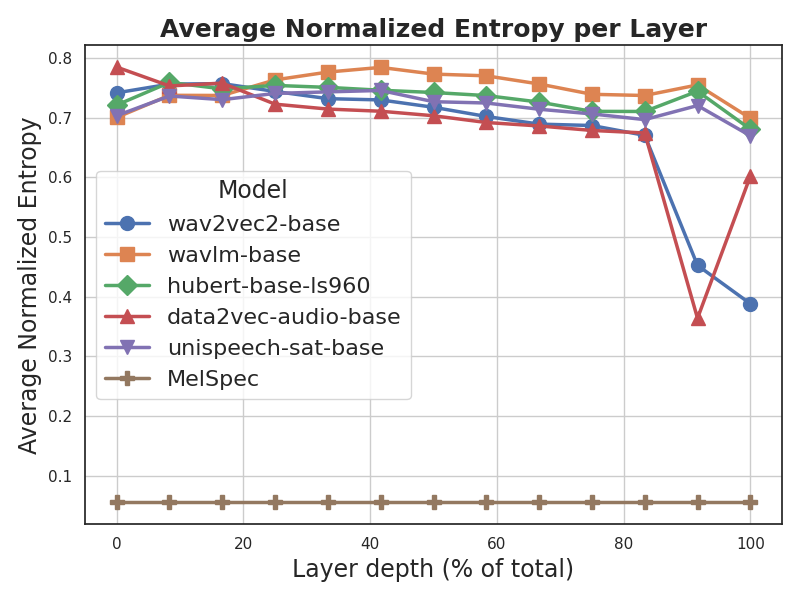
\includegraphics[width=\textwidth]{figures/exp-1/entropy.png}
        \caption{Entropy}
        \label{fig:fig1}
    \end{subfigure}
    \hfill
    % Deuxième sous-figure
    \begin{subfigure}[b]{0.32\textwidth}
        \centering
        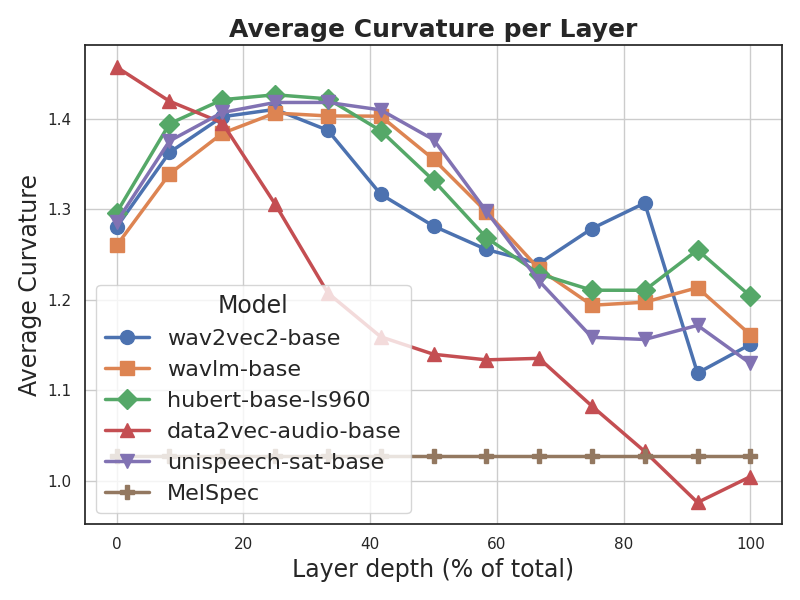
\includegraphics[width=\textwidth]{figures/exp-1/curvature.png}
        \caption{Curvature}
        \label{fig:fig2}
    \end{subfigure}
    \hfill
    % Troisième sous-figure
    \begin{subfigure}[b]{0.32\textwidth}
        \centering
        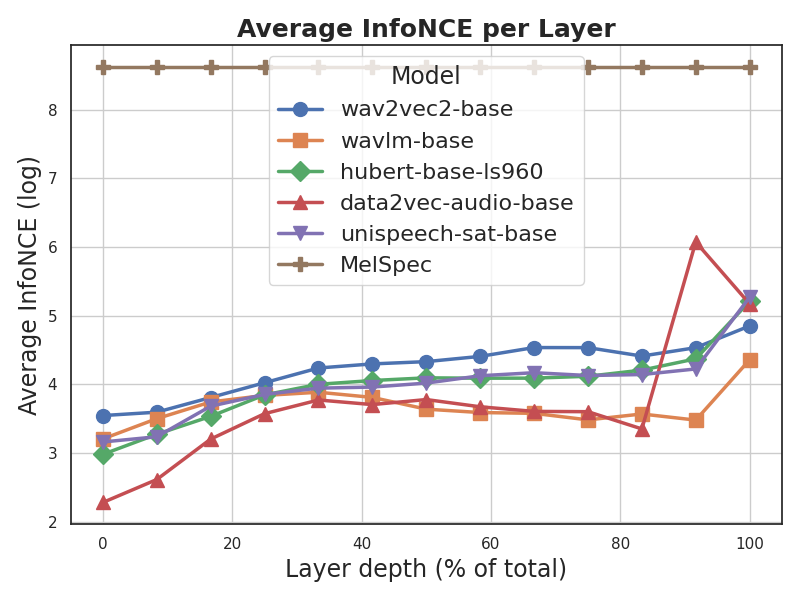
\includegraphics[width=\textwidth]{figures/exp-1/invariance.png}
        \caption{InfoNCE}
        \label{fig:fig3}
    \end{subfigure}
    
    \caption{Layer-wise analysis of SSL models across three complementary perspectives: information-theoretic (entropy), geometric (curvature), and invariance (robustness to input perturbations).}
    \label{fig:analysis-3-perspectives}
\end{figure*}

\begin{figure*}[t]
    \centering
    % Première sous-figure
    \begin{subfigure}[b]{0.32\textwidth}
        \centering
        
\includegraphics[width=\textwidth]{figures/size/0.png}
        \caption{Entropy}
        \label{fig:fig1}
    \end{subfigure}
    \hfill
    % Deuxième sous-figure
    \begin{subfigure}[b]{0.32\textwidth}
        \centering
        
\includegraphics[width=\textwidth]{figures/size/1.png}
        \caption{Curvature}
        \label{fig:fig2}
    \end{subfigure}
    \hfill
    % Troisième sous-figure
    \begin{subfigure}[b]{0.32\textwidth}
        \centering
        
\includegraphics[width=\textwidth]{figures/size/2.png}
        \caption{InfoNCE}
        \label{fig:fig3}
    \end{subfigure}
    
    \caption{The impact of training data and model size on SSL representations, showing how layer-wise properties—entropy, curvature, and invariance—vary across models of different scales.}
    \label{fig:size}
\end{figure*}

\begin{figure*}[t]
    \centering
    % Première sous-figure
    \begin{subfigure}[b]{0.32\textwidth}
        \centering
        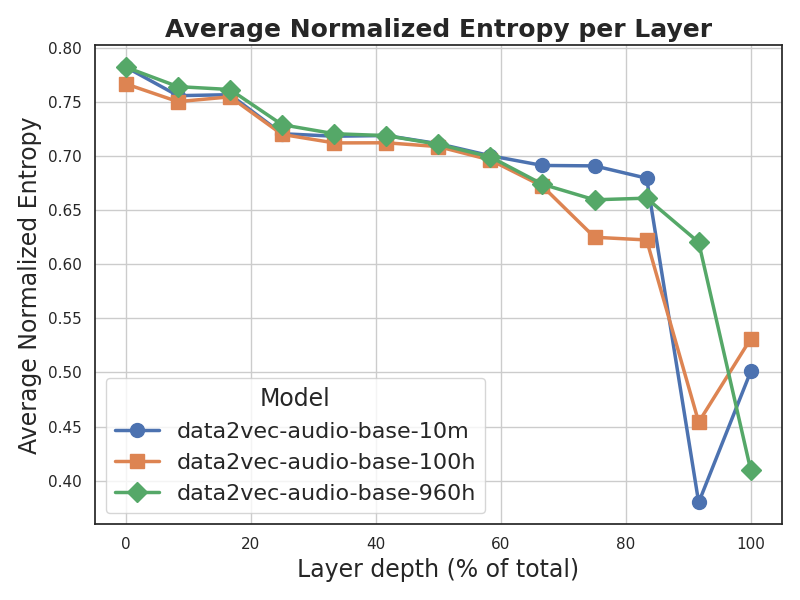
\includegraphics[width=\textwidth]{figures/finetune/0.png}
        \caption{Entropy}
        \label{fig:fig1}
    \end{subfigure}
    \hfill
    % Deuxième sous-figure
    \begin{subfigure}[b]{0.32\textwidth}
        \centering
        
\includegraphics[width=\textwidth]{figures/finetune/1.png}
        \caption{Curvature}
        \label{fig:fig2}
    \end{subfigure}
    \hfill
    % Troisième sous-figure
    \begin{subfigure}[b]{0.32\textwidth}
        \centering
        
\includegraphics[width=\textwidth]{figures/finetune/2.png}
        \caption{InfoNCE}
        \label{fig:fig3}
    \end{subfigure}
    
    \caption{Effect of fine-tuning on SSL audio representations, illustrating how layer-wise properties—entropy, curvature, and invariance—change after task-specific adaptation.}
    \label{fig:finetune}
\end{figure*}

\subsection{Geometric Analysis}

Following \cite{hosseini2023large}, we analyze the embeddings from a geometric perspective by focusing on their \textbf{curvature}.  
As introduced in Section~\ref{sec:notation}, curvature captures how sharply token embeddings turn along a sequence.  
It allows us to distinguish between local, fine-grained variations (high curvature) and smoother, globally consistent structures (low curvature).  
By tracking curvature across layers, we gain insight into how SSL models transition from encoding local acoustic details to representing higher-level semantic information.

A decrease in curvature indicates that representations follow smoother, more linear trajectories, consistent with the abstraction of higher-level semantic information. In contrast, higher curvature reflects locally complex trajectories, capturing fine-grained acoustic or phonetic details. This connection suggests that curvature is not only a geometric property but also an indicator of the representational content, bridging the transition from low-level signal encoding to more abstract, semantically meaningful structures across layers.

\subsection{Augmentation invariance metrics}

To systematically measure robustness, we evaluate the embeddings of augmented audio samples using InfoNCE \citep{oord2018representation}, a contrastive loss where a lower value indicates stronger invariance. In practice, this metric encourages embeddings of augmented versions of the same audio to be closer together while pushing apart embeddings from different audio samples, providing a clear measure of the model's ability to learn invariant representations.

% \begin{itemize}
%     \item \textbf{InfoNCE} \citep{oord2018representation}: a contrastive loss where a lower value indicates stronger invariance.  
%     \item \textbf{LiDAR} \citep{thilak2023lidar}: treats each audio segment as a class and measures the tightness of clusters under augmentation.  
%     \item \textbf{DiME} \citep{skean2023dime}: compares embeddings of true augmented pairs against random pairings to evaluate alignment and invariance.
% \end{itemize}

\subsection{Layer-by-Layer comparison}

By combining these three analytical perspectives, we can characterize the function of each layer in complementary ways. Some layers act as efficient compressors, reducing redundancy while preserving task-relevant information. Others reveal well-structured manifold geometry, capturing the organization of embeddings in the representation space. Still others demonstrate strong robustness to perturbations, ensuring stability under input variations. Altogether, this methodology provides a comprehensive, layer-wise understanding of how SSL audio models, such as WavLM and Wav2Vec, encode, organize, and stabilize their representations.

\paragraph{Connecting the three perspectives}
Although each perspective (information-theoretic, geometric, and invariance) offers distinct insights, they are inherently \emph{interconnected}.
The degree of information compression influences the geometric structure of embeddings: excessive compression can collapse the representation space, while balanced compression yields well-organized manifolds.
Similarly, a structured geometry facilitates invariance by ensuring that perturbations do not drastically distort representations.
Conversely, robustness to perturbations reinforces both compression and geometry, since stable embeddings retain meaningful information across conditions.
Taken together, these perspectives form a coherent framework to assess how SSL models progressively transform raw acoustic inputs into robust and semantically organized representations.


\section{Experiments}
\subsection{Experimental Setup}
We evaluate our methodology on several widely used SSL models. For each model, we extract hidden representations at every layer and analyze them according to the three perspectives described in Section~\ref{sec:methodology}: (i) information-theoretic, (ii) geometric, and (iii) invariance.  

\paragraph{Models} All the studied  Self-Supervised Learning models in this paper utilize a bidirectional Transformer architecture, but their pre-training objectives vary significantly: Wav2Vec 2.0 learns contextualized representations by masking latent speech units and employing a contrastive prediction task to discriminate the true unit from negatives. HuBERT follows a similar masked prediction objective but relies on offline clustering to generate discrete pseudo-labels for the masked units, enabling iterative refinement. WavLM extends HuBERT's approach by incorporating additional denoising and speech separation objectives, specifically designed to improve robustness in noisy and multi-speaker environments. Finally, Data2Vec Audio is distinguished by its modality-agnostic teacher–student framework, where it learns to predict the continuous latent representations from the teacher network rather than discrete units, offering a different pathway to self-supervision. 

\paragraph{Data} Unless otherwise specified, experiments are conducted on the \textbf{Librispeech} corpus (train-clean-100 subset) to ensure consistent comparisons across models.  

\paragraph{Augmentations} To assess invariance, we generate two augmented versions of each audio segment using common perturbations: additive Gaussian noise, time masking, pitch shifting, and time-stretching.  

\paragraph{Implementation details} All embeddings are computed with the official checkpoints. For information-theoretic metrics, we compute matrix-based entropy with $\alpha=1$ (von Neumann entropy).


\subsection{Analysis of SSL Models Across the Three Perspectives (Figure~\ref{fig:analysis-3-perspectives})}

\paragraph{Information-Theoretic Perspective} Representations based on the Mel-Spectrogram exhibit the lowest entropy (brown line), as they capture raw acoustic features lacking the richness of contextual and semantic information. Conversely, all SSL models maintain high and stable entropy in the input and intermediate layers (around 0.75), indicating a richness of information and low initial compression of the embeddings. WavLM, UniSpeech-sat, and HuBERT models show a slight tendency towards compression (entropy drop) in the final layers (around 90-100\% depth), suggesting a filtering process that retains relevant semantic information while discarding acoustic redundancy. Data2vec-audio and Wav2vec2 show an even more pronounced compression, with a noticeable drop in entropy in the deepest layers.

% Interestingly, this drop in entropy aligns with findings from a large-scale probing analysis by \cite{chiu2025probing}, which observed a substantial decrease in speaker-specific information in the final layers of these models as illustrated in Figure~\ref{fig:tasks}. Specifically, the study found that intermediate layers effectively capture a mix of acoustic and para-linguistic information, with deeper layers refining these representations.

% This correlation suggests that the compression observed in the final layers may be associated with the model's focus on abstracting linguistic content, potentially at the expense of speaker identity information.

\paragraph{Geometric Perspective} The Mel-Spectrogram shows extremely low curvature (brown line, around 1.05), indicating very smooth and linear token trajectories without the complexity of linguistic structures. SSL models exhibit a clear transformation pattern: they display high curvature in the initial and intermediate layers (peaking around 30-50\% depth, near 1.40). This high curvature is associated with capturing local, fine-grained acoustic and phonetic details (abrupt changes between tokens). The curvature significantly decreases in the deep layers (around 1.15-1.20), reflecting a transition toward smoother and more linear representations. This is characteristic of building global semantic structures and linguistic coherence. 

\paragraph{Augmentation Invariance Perspective} The Mel-Spectrogram predictably shows the highest InfoNCE (over 8.0, off-scale in Figure 1c), indicating that it is extremely sensitive to input perturbations and fails to learn invariant representations (a characteristic of raw features). All SSL models demonstrate strong invariance in the initial layers (low InfoNCE, around 3.0), meaning these layers are very robust, and input variations (augmentations) do not significantly alter the acoustic embeddings. InfoNCE steadily increases for all SSL models as they progress toward the output layers. This increase (showing a decrease in invariance) is particularly notable for Wav2vec2-Base, suggesting that its deep layers are more sensitive to the details introduced by augmentation. WavLM maintains a more moderate InfoNCE growth, implying that their pre-training mechanisms (like WavLM's contrastive training) enable them to build final semantic representations that remain relatively more stable against perturbations than other models.


\subsection{Influence of training data size and model Size (Figure~\ref{fig:size})} The analysis of WavLM representations reveals that increasing the training data size (Base vs. Base-Plus) has minimal impact on embedding structure, while scaling the model size (Base-Plus vs. Large) fundamentally alters the representation strategy. From an information-theoretic (Entropy) perspective, the Base and Base-Plus versions maintain high and nearly identical entropy profiles (around 0.75-0.78), signifying high information richness. In contrast, WavLM-Large displays significantly lower entropy (around 0.55-0.65), indicating more effective and earlier information compression, as the larger model concentrates essential information into a smaller variance subspace. Geometrically (Curvature), Base and Base-Plus both show the same sharp curvature  peak in the mid-layers (around 40\% depth, near 1.40), followed by a steep drop, symbolizing a rapid transition from local acoustic details to global semantic structures. WavLM-Large, however, exhibits a flatter, overall lower curvature profile with a notable late second peak, suggesting a more stable processing of local features and a possible re-encoding of fine-grained interactions in the deeper layers. Finally, the invariance (InfoNCE) metric reveals the most striking  contrast: WavLM-Base and WavLM-Base-Plus maintain very high robustness (low and stable InfoNCE), which is beneficial for speaker-related tasks. WavLM-Large, conversely, displays a drastically high InfoNCE in its intermediate layers (peaking at 13.0), signaling a severe loss of invariance and high sensitivity to input perturbations. This suggests that the Large model, while informationally efficient, compromises robustness, although there is an abrupt drop in InfoNCE in the final layer, likely serving as a regularization step for the output.

The sharp drop in InfoNCE at the final layer of WavLM-Large is a critical observation, suggesting that the model, despite accumulating low invariance in deep layers due to learning highly specific features, employs its output layer as a strong final regularization or projection head. This abrupt reduction forces the embeddings of augmented pairs to converge again, effectively restoring high invariance just before the output to ensure the final representation is robust and usable for downstream tasks. This represents a trade-off where complex intermediate layers prioritize discrimination, and the final layer corrects for robustness. We hypothesize that the low Normalized Entropy observed in the intermediate layers of WavLM-Large is causally linked to its significantly high InfoNCE. Low entropy reflects aggressive information compression, wherein the high-capacity model efficiently concentrates crucial semantic features into a highly dense, low-dimensional subspace. This efficiency, however, introduces representational fragility: the lack of informational redundancy within this compressed manifold means that a minor input perturbation (augmentation) can easily displace the embedding from its narrowly optimized location. Consequently, the representations of augmented pairs are perceived as distinct, resulting in the high InfoNCE, thereby indicating a compromise of invariance in favor of maximal feature discrimination within the latent space.

\subsection{Influence of Fine-Tuning (Figure~\ref{fig:finetune})} 
The increase in the amount of fine-tuning data (from 10m to 960h) drives both specialization and regularization in the data2vec-audio-base representations. Regarding Entropy, the 960h model (green) achieves the most effective information compression and earliest specialization (lowest overall entropy), whereas the 100h model (orange) retains the highest average redundancy. Geometrically (Curvature), the ample 960h data prevents the drastic curvature drop seen with 10m (blue), allowing the model to maintain a complex, non-linear geometric structure in the deep layers, essential for semantic encoding. Crucially, in terms of Invariance (InfoNCE), the 960h model exhibits the highest robustness (lowest InfoNCE) in deep layers, confirming that large-scale fine-tuning acts as a powerful regularizer that preserves stability against perturbations.

\subsection{Connection to speech tasks}
\begin{figure*}
    \centering
    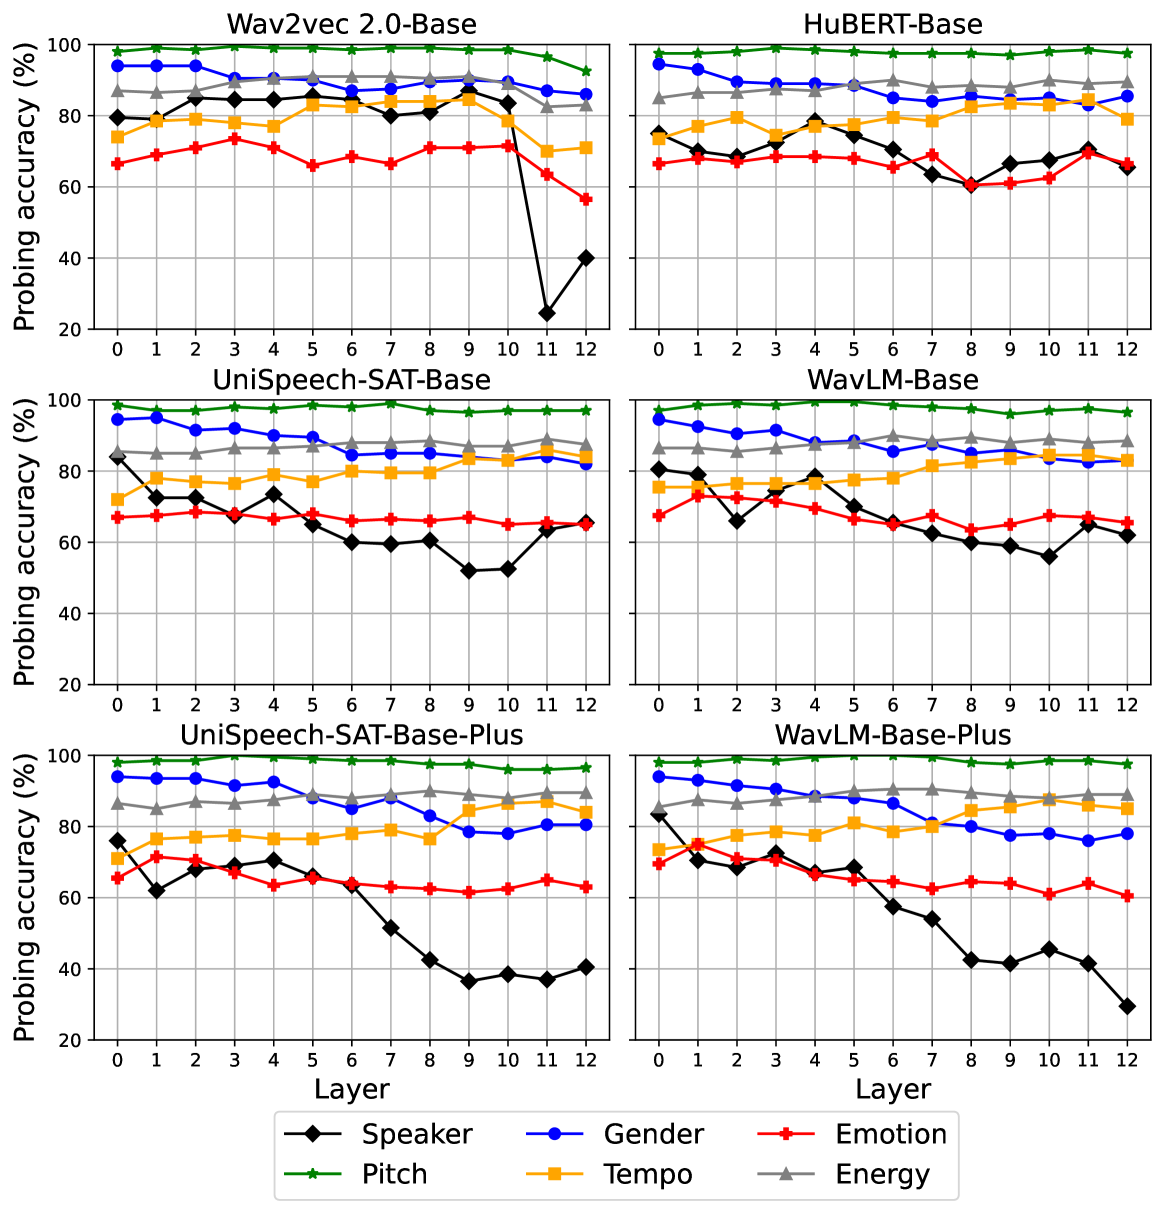
\includegraphics[width=1\linewidth]{figures/x3.png}
    \caption{Probing accuracies of the Base and Base Plus variants of speech SSL models on the test set (taken from \citep{chiu2025probing}).}
    \label{fig:tasks}
\end{figure*}

\bibliography{mybibfile}
% \balance

\end{document}